\documentclass{beamer}

% Theme choice:
\usetheme{CambridgeUS}
\usepackage{amsmath}
\usepackage{mathtools}
\providecommand{\pr}[1]{\ensuremath{\Pr\left(#1\right)}}
\providecommand{\cdf}[2]{\ensuremath{\text{F}_{#1}\left(#2\right)}}
\providecommand{\erf}[1]{\ensuremath{\text{erf}(#1)}}
\setbeamertemplate{caption}[numbered]
% Title page details: 
\title{Parameteres for financial health of a bank} 
\author{Lokesh Surana (ES20BTECH11017)}
\date{\today}

\begin{document}

% Title page frame
\begin{frame}
    \titlepage 
\end{frame}

% Outline frame
\begin{frame}{Outline}
    \tableofcontents
\end{frame}

\section{Previous presentation}
\begin{frame}{Previous presentation}
	\textbf{(Financial health of a bank)} Can we assess the financial health of a bank using publicly availalbe balancesheets and information?
	\begin{enumerate}
		\item We discussed on what all types of risk are there for banks - Credit Risk, Operational Risk, Market Risk, Liquidity Risk.
		\item And then we've seen some of the key financial ratios and their signficance - Net NPA, Net interest margin, Loan-to-Assets ratio, Return-to-assests ratio, CASA ratio, Capital adequacy ratio
	\end{enumerate}
\end{frame}

\section{Problems}
\begin{frame}{Problems}
	\textbf{There were some questions raised in the previous presentation:}
	\begin{enumerate}
		\item What are the healty ranges for these financial ratios for any bank?
		\item Is CASA ratio really a good indicator of financial health of a bank?
		\item In Capital adequacy ratio - What are the Tier1 and Tier2 capital? What are the risk weighted assets?
	\end{enumerate}
	Let's look into all of these using publicly available data.
\end{frame}

\subsection{Healthy ranges for financial ratios}
\begin{frame}{Financial Ratio Range - Net NPA}
	Lets observe the Net NPA ratio for some of the banks in India.
	\begin{figure}
		\centering
		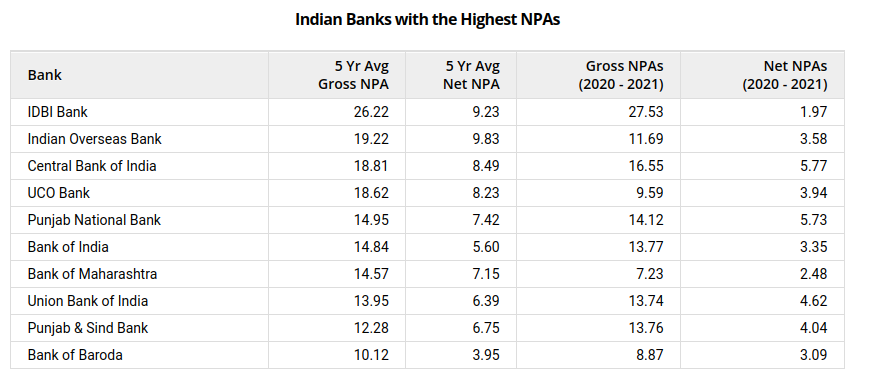
\includegraphics[width=0.7\linewidth]{Highest NPA.png}
		\label{fig:netnpa}
	\end{figure}
\end{frame}

\begin{frame}{Financial Ratio Range - Net NPA}
	\begin{figure}
		\centering
		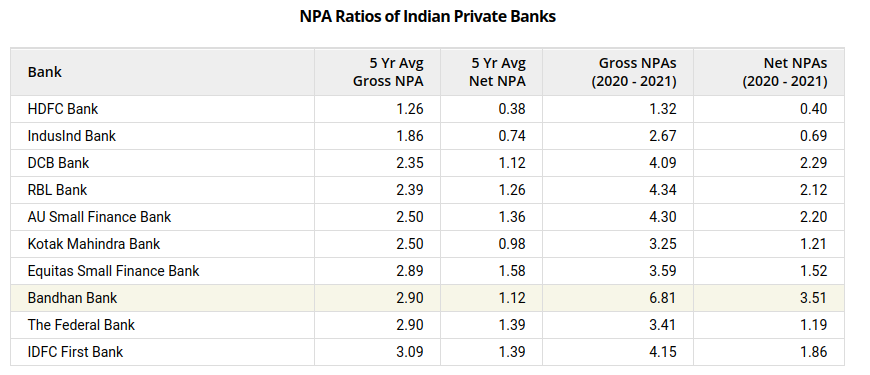
\includegraphics[width=0.7\linewidth]{Private banks NPA.png}
		\label{fig:netnpapvt}
	\end{figure}
	Net NPA is lower the better, and ideally with Net NPA less than 2\% is considered healthy.
\end{frame}

\begin{frame}{Return to assets}
	\begin{enumerate}
		\item The return-on-assets (ROA) ratio is frequently applied to banks because the cash flow analysis is more difficult to accurately construct. The ratio is considered an important profitability ratio, indicating the per-rupee profit a company earns on its assets. 
		\item Since bank assets largely consist of money the bank loans, the per-rupee return is an important metric of bank management. The ROA ratio is a company's net, after-tax income divided by its total assets. 
		\item An important point to note is since banks are highly leveraged, even a relatively low ROA of 1 to 2\% may represent substantial revenues and profit for a bank.
	\end{enumerate}
\end{frame}

\begin{frame}{CASA ratio}
	\begin{figure}
		\centering
		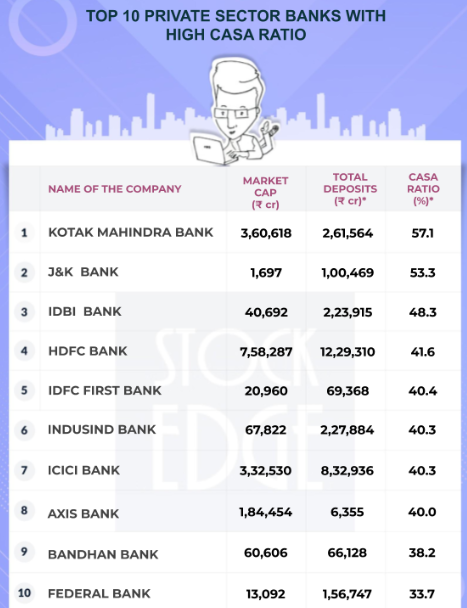
\includegraphics[width=0.47\linewidth]{CASAratio.png}
		\label{fig:casa}
	\end{figure}
\end{frame}

\subsection{CASA ratio}
\begin{frame}{CASA ratio}
	\begin{enumerate}
		\item CASA Ratio = CASA Deposits ÷ Total Deposits
		\item The CASA is a non-term deposit, meaning it is used for the everyday banking and savings needs of the consumer. This type of account does not have a specific maturity or expiration date, so it is valid for as long as the account holder needs it to remain open.
		\item Financial institutions encourage the use of a CASA because it generates a higher profit margin. Because the interest paid on the CASA deposit is lower than on a term deposit, the bank’s net interest income is higher. Thus, CASAs can be a cheaper source of funding for banks.
		\item \textbf{However, because of the uncertainty relating to when a depositor will withdraw funds, CASA funds should not be utilized by a bank for long-term financing.}
	\end{enumerate}
\end{frame}

\subsection{Capital adequacy ratio}
\begin{frame}{Capital adequacy ratio}
	\begin{enumerate}
		\item Capital adequacy ratio (CAR) is a measure of a bank's available capital expressed as a percentage of a bank's risk-weighted credit exposures.
		\item CAR = $\frac{\text{Tier 1 Capital + Tier 2 Capital}}{\text{risk-weighted asset}}$
	\end{enumerate}
\end{frame}

\begin{frame}{Tier1 and Tier2 assests}
	\begin{enumerate}
		\item Tier I Capital: consists mainly of share capital and etained earnings—disclosed on their financial statements. Since this capital is fully available to cover the core losses, it is also called Core Capital. For this reason this is considered as the highest quality capital. hese funds are generated specifically to support banks when losses are absorbed so that regular business functions do not have to be shut down.
		\item Tier II Capital (supplementary capital): Includes undisclosed funds that do not appear on a bank's financial statements, revaluation reserves, hybrid capital instruments, subordinated term debt. It is more difficult to accurately measure due to its composition of assets that are difficult to liquidate.
	\end{enumerate}
\end{frame}

\begin{frame}{Risk weighted assests}
	\begin{enumerate}
		\item Regulators ask each bank must group its assets together by risk category so that the amount of required capital is matched with the risk level of each asset type. Basel III uses credit ratings of certain assets to establish their risk coefficients. 
		\item The degree of risk involved is expressed in percentage and it is assigned by the Reserve Bank of India. The Risk weights of a few important assets as assigned by the RBI are listed in the table below:
	\end{enumerate}
\end{frame}

\begin{frame}
	\begin{figure}
		\centering
		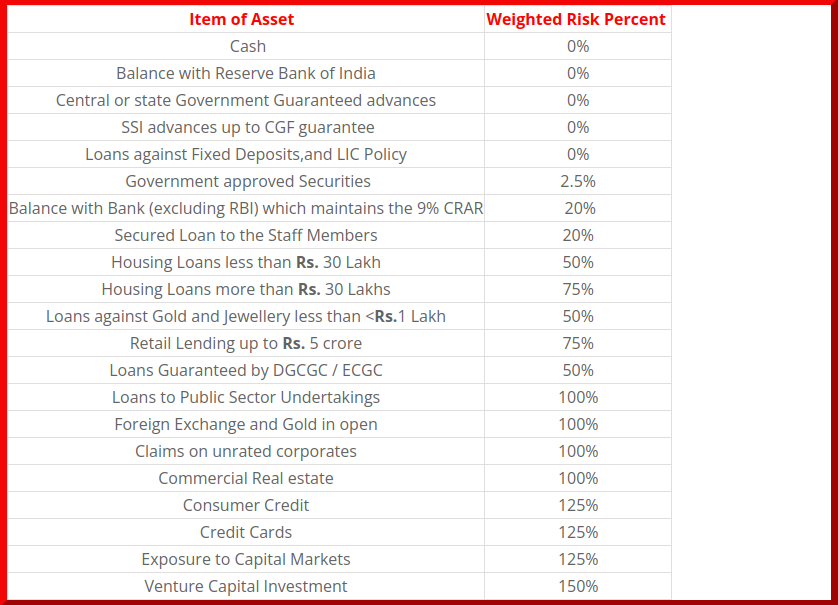
\includegraphics[width=0.7\linewidth]{Risk_weighted_assets.png}
		\caption{Risk weighted assets}
		\label{fig:riskweightedassets}
	\end{figure}
\end{frame}

\end{document}